\documentclass[aps,prd,twocolumn,superscriptaddress,nofootinbib,floatfix]{revtex4-2}

\usepackage{amsmath,amssymb,amsthm,mathtools}
\usepackage[T1]{fontenc}
\usepackage{lmodern}
\usepackage{tikz}
\usetikzlibrary{arrows.meta,positioning,calc}
\usepackage{pgfplots}
\pgfplotsset{compat=1.18}
\usepackage{booktabs}
\usepackage{array}
\usepackage[colorlinks=true,linkcolor=blue,citecolor=red,urlcolor=blue]{hyperref}

\newtheorem{theorem}{Theorem}
\newtheorem{proposition}[theorem]{Proposition}
\newtheorem{lemma}[theorem]{Lemma}
\newtheorem{corollary}[theorem]{Corollary}
\theoremstyle{definition}
\newtheorem{definition}[theorem]{Definition}
\newtheorem{hypothesis}[theorem]{Hypothesis}
\theoremstyle{remark}
\newtheorem{remark}[theorem]{Remark}

\DeclareMathOperator{\SU}{SU}
\DeclareMathOperator{\U}{U}
\DeclareMathOperator{\Tr}{tr}
\DeclareMathOperator{\osc}{osc}
\DeclareMathOperator{\Var}{Var}
\DeclareMathOperator{\Ent}{Ent}
\DeclareMathOperator{\Ric}{Ric}
\newcommand{\cO}{\mathcal{O}}
\newcommand{\cH}{\mathcal{H}}
\newcommand{\cA}{\mathcal{A}}
\newcommand{\cB}{\mathcal{B}}
\newcommand{\cG}{\mathcal{G}}
\newcommand{\R}{\mathbb{R}}
\newcommand{\Z}{\mathbb{Z}}
\newcommand{\Dlat}{\Delta_{\mathrm{lat}}}

\begin{document}
\emergencystretch=3em\hbadness=10000

\title{Spacing-Uniform Lattice Inequalities Cannot Produce the Yang--Mills Mass Gap}

\author{Deep Bhattacharjee}
\email{itsdeep@live.com}
\thanks{Corresponding author.}
\affiliation{Formerly, Electro-Gravitational Space Propulsion Laboratory (EGSPL), Bhubaneswar, Odisha 751030, India}
\affiliation{Formerly, University of Calcutta, 87/1 College Street, Kolkata 700073, India}

\author{Ushashi Bhattacharya}
\email{rai.bhattacharya.in@gmail.com}
\affiliation{Formerly, National Taiwan University, Taipei 106319, Taiwan}

\date{\today}

\begin{abstract}
We prove that a family of reflection-positive lattice gauge theories whose
transfer matrices have a spectral gap bounded below in lattice units,
uniformly in the spacing, has renormalised two-point functions whose limits
vanish at every temporal separation after the first one at which a limit
exists, so that it cannot converge to a continuum theory with a finite
positive mass gap. Spacing-uniform log-Sobolev, Poincar\'e, Dobrushin and
clustering bounds are therefore excluded as routes to the Yang--Mills
existence and mass-gap problem. We prove three further obstructions: global
Holley--Stroock perturbation of Haar measure by the Wilson weight loses the
factor $e^{-2N\beta|P|}$; bounded nonnegative plaquette terms do not bound
the free-energy cumulants uniformly in the volume, and plaquette variables
satisfy exact Bianchi relations in dimension three or more; the one-loop
effective coupling takes every positive value at a scale independent of the
spacing, so no continuum limit avoids intermediate coupling. Every one of
these statements is checked in Lean~4 with Mathlib, with every proof complete
and no axiom beyond the three standard ones. We use them to locate the
errors of eight manuscripts that claimed the mass gap by this route, we
record what is known unconditionally, and we state the single residual
statement that separates it from the Clay problem. The problem remains open.
\end{abstract}

\maketitle

\tableofcontents

\section{Introduction}
\label{sec:intro}

The Yang--Mills existence and mass-gap problem~\cite{JW00} asks for a
quantum $\SU(N)$ gauge theory on $\R^4$ satisfying the Wightman or
Osterwalder--Schrader axioms~\cite{OS73,OS75,GJ87} whose Hamiltonian has
spectrum $\{0\}\cup[\Delta,\infty)$ with $\Delta>0$. The standard starting
point is Wilson's lattice theory~\cite{Wil74}. For spacing $a>0$ and
coupling $\beta=2N/g^2$ the Wilson measure on $\SU(N)$-valued link variables
is reflection positive~\cite{OSei78}, so it has a positive transfer matrix
$T_a$ and a lattice Hamiltonian $-\log T_a$; at strong coupling (small
$\beta$) convergent expansions give a transfer-matrix gap and exponential
clustering~\cite{OSei78,Sei82,KP86}. The unsolved content is the continuum
limit $a\to0$ along the asymptotic-freedom trajectory $\beta(a)\to\infty$.

Between 2025 and 2026 the authors circulated eight manuscripts (preprints
226502, 226913, 227159, 227445, 228638 and 229061, two of them in two
copies) built on one strategy: a lower bound on the Bakry--\'Emery curvature
of the gauge-orbit space~\cite{BE85,Mil76}, transferred to the Wilson
measure by Holley--Stroock perturbation~\cite{HS87} and
Dobrushin--Stroock--Zegarlinski assembly~\cite{SZ92}, gives a log-Sobolev
constant uniform in the volume and the spacing, hence a uniform lattice gap,
hence a continuum mass gap. The last of the eight, 229061, already observed
that this strategy defeats itself. The present paper replaces those
manuscripts. It proves that observation in a stronger form, adds three
further obstructions, checks all four in Lean, and lists the errors of the
earlier texts by file and line.

\begin{theorem}[No-go; Theorem~\ref{thm:nogo}]
\label{thm:A}
Let lattice theories indexed along any family of spacings $a\to0^+$ have
transfer-matrix gaps $\Dlat(a)\ge\delta>0$ in lattice units. For every
choice of gauge-invariant observables and renormalisations $Z_a>0$, if the
renormalised temporal two-point functions converge at separations
$0\le t_1<t_2$, the limit at $t_2$ is zero. No such family converges to the
two-point function of a continuum theory with gap $\Delta\in(0,\infty)$
and a nonzero spectral measure.
\end{theorem}

\begin{theorem}[Volume obstruction; Proposition~\ref{prop:volume}]
\label{thm:B}
For $U\in\U(N)$, $|\mathrm{Re}\Tr U|\le N$. The Wilson action over a set
$P$ of plaquettes has oscillation at most $2N|P|$, and the Holley--Stroock
factor $e^{-2N\beta|P|}$ tends to zero as $|P|\to\infty$ at every
$\beta>0$.
\end{theorem}

\begin{theorem}[Cumulants and Bianchi; Section~\ref{sec:cumulant}]
\label{thm:C}
There are actions that are sums of $n$ local terms in $[0,2N]$ with
$\Var(S_n)/n=N^2n$. On every unit cube the six oriented plaquette angles of
an abelian configuration sum to zero.
\end{theorem}

\begin{theorem}[The window is entered; Section~\ref{sec:running}]
\label{thm:D}
The one-loop coupling $g^2(\mu)=1/(2b_0\log(\mu/\Lambda))$,
$b_0=11N/(48\pi^2)$, takes every value $g_*^2>0$ at
$\mu_*=\Lambda\exp(1/(2b_0g_*^2))$, a scale independent of $a$ and inside
$(\Lambda,1/a)$ for every $a<1/\mu_*$.
\end{theorem}

Theorems~\ref{thm:A} to~\ref{thm:D} are checked in Lean~4, as described in
Section~\ref{sec:lean}. Together they show where each of the earlier
manuscripts fails (Section~\ref{sec:audit}): the curvature step proves too
little (it controls only Haar measure, or strong coupling), the analyticity
step uses an independence that is false in four dimensions, the coupling
step assumes that the continuum limit avoids intermediate coupling, which is
impossible, and the final step, a gap uniform in the spacing, would refute
the goal it was meant to prove.

Section~\ref{sec:known} records what is known unconditionally, and
Section~\ref{sec:claims} examines the other claimed proofs we found.
Section~\ref{sec:residual} states the residual statement. The paper proves
no existence or gap statement for the continuum theory.

\section{Setting}
\label{sec:setting}

Fix $N\ge2$. For a finite hypercubic lattice $\Lambda\subset a\Z^4$ with
links $E$ and plaquettes $P$, the Wilson measure is
\begin{align}
d\mu_{\Lambda,\beta}(U)&=Z^{-1}e^{-\beta S(U)}\prod_{e\in E}dU_e,\nonumber\\
S(U)&=\sum_{p\in P}\bigl(N-\mathrm{Re}\Tr U_p\bigr),
\label{eq:wilson}
\end{align}
with $dU_e$ normalised Haar measure and $U_p$ the ordered product of links
around $p$. Reflection positivity in temporal planes~\cite{OSei78} gives a
Hilbert space $\cH_a$, a self-adjoint transfer matrix $0\le T_a\le1$ with
ground state $\Omega_a$, and for a gauge-invariant observable $\cO_a$
localised in a time slice the spectral representation of the truncated
temporal two-point function at $t\in a\Z_{>0}$:
\begin{equation}
S_a(t)=\int_{[0,\infty)}e^{-Et/a}\,d\rho_a(E),
\label{eq:spectral}
\end{equation}
where $E$ runs over the spectrum of $-\log T_a$ (lattice units) on the
orthogonal complement of $\Omega_a$ and $\rho_a$ is the spectral measure of
$(\cO_a-\langle\cO_a\rangle)\Omega_a$, a finite positive measure. A lattice
gap $\Dlat(a)\ge\delta$ means $\rho_a([0,\delta))=0$ for all such
observables. Formula~\eqref{eq:spectral} defines $S_a(t)$ for every real
$t\ge0$; along any sequence of spacings for which $t\in a\Z$ it is the
lattice two-point function, and the theorems below are stated along an
arbitrary filter so that they apply to every such sequence.

The physical gap of the lattice theory is $\Dlat(a)/a$. A continuum theory
with mass $m$ requires $\Dlat(a)=ma+o(a)$; the earlier manuscripts wrote
$\Delta_a$ for $\Dlat(a)$ and then treated it alternately as a lattice-unit
and a physical quantity (Section~\ref{sec:audit}).

\section{The no-go theorem}
\label{sec:nogo}

\begin{lemma}[Ratio bound]
\label{lem:ratio}
If $\rho$ is a finite positive measure with $\rho([0,\delta))=0$, $\delta\ge0$,
$a>0$ and $0\le t_1\le t_2$, then
\begin{equation}
S_a(t_2)\le e^{-\delta(t_2-t_1)/a}\,S_a(t_1).
\label{eq:ratio}
\end{equation}
\end{lemma}

\begin{proof}
On the support $E\ge\delta$, so
$e^{-Et_2/a}=e^{-E(t_2-t_1)/a}e^{-Et_1/a}\le
e^{-\delta(t_2-t_1)/a}e^{-Et_1/a}$; both integrands are bounded by $1$ on
the support, hence integrable for the finite measure $\rho$; integrate.
\end{proof}

Every renormalisation constant cancels in~\eqref{eq:ratio}, and its right
side carries the factor $e^{-c/a}$, $c=\delta(t_2-t_1)>0$.

\begin{theorem}[Spacing-uniform gaps force ultralocal limits]
\label{thm:nogo}
Let $(a_i)$ tend to $0^+$ along a filter, let $\rho_i$ be finite positive
measures with $\rho_i([0,\delta))=0$ for a fixed $\delta>0$, and let
$Z_i>0$. If $Z_iS_{a_i}(t_1)\to L_1$ and $Z_iS_{a_i}(t_2)\to L_2$ with
$0\le t_1<t_2$, then $L_2=0$.
\end{theorem}

\begin{proof}
By~\eqref{eq:ratio},
$0\le Z_iS_{a_i}(t_2)\le e^{-c/a_i}\,Z_iS_{a_i}(t_1)$. The first factor
tends to $0$ and the second to $L_1$, so the middle term tends to $0$.
\end{proof}

The statement is stronger than the one in 229061, which assumed $L_1\ne0$:
convergence at the earlier time alone forces the later limit to vanish.

\begin{lemma}[K\"all\'en--Lehmann positivity]
\label{lem:KL}
If $\sigma\ne0$ is a finite positive measure with $\sigma([0,\Delta))=0$,
$\Delta>0$, then $S(t)=\int e^{-Et}d\sigma(E)>0$ for every $t>0$.
\end{lemma}

\begin{proof}
The integrand is strictly positive and bounded by $1$ on the support, and
$\sigma(\R)>0$.
\end{proof}

\begin{corollary}
\label{cor:nogap}
Under the hypotheses of Theorem~\ref{thm:nogo}, the renormalised two-point
functions cannot converge at every $t>0$ to the two-point function of a
continuum theory with gap $\Delta>0$ and nonzero spectral measure. If
$\Dlat(a)/a\to m$, then $\Dlat(a)\to0$, so no $\delta>0$ bounds $\Dlat$
below.
\end{corollary}

\begin{proof}
Apply Theorem~\ref{thm:nogo} with $t_1=1$, $t_2=2$: the limit at $t=2$
would be $0$, against Lemma~\ref{lem:KL}. For the second statement,
$\Dlat(a)=(\Dlat(a)/a)\,a\to m\cdot0$.
\end{proof}

\begin{lemma}[Critical scaling]
\label{lem:critical}
Let $(a_i)$ tend to $0^+$ along a filter, let $\rho_i$ be finite positive
measures with $\rho_i([0,m_ia_i))=0$ for numbers $m_i\ge0$ with $m_i\to m$,
and let $Z_i>0$. If $Z_iS_{a_i}(t_1)\to L_1$ and $Z_iS_{a_i}(t_2)\to L_2$ with
$0\le t_1\le t_2$, then $L_2\le e^{-m(t_2-t_1)}L_1$.
\end{lemma}

\begin{proof}
Lemma~\ref{lem:ratio} with $\delta=m_ia_i$ gives
$Z_iS_{a_i}(t_2)\le e^{-m_i(t_2-t_1)}Z_iS_{a_i}(t_1)$; the right side tends
to $e^{-m(t_2-t_1)}L_1$.
\end{proof}

Lemma~\ref{lem:critical} is the bound that Theorem~\ref{thm:nogo} leaves
open. A lattice gap bounded below by a constant is excluded; a lattice gap
bounded below by $ma$ makes every limiting two-point function satisfy the
ratio bound of a theory with gap $m$, and a Laplace transform of a finite
positive measure obeying $S(t_2)\le e^{-m(t_2-t_1)}S(t_1)$ for all
$t_1\le t_2$ has its measure supported in $[m,\infty)$. The converse does
not follow from anything here: a gapped limit forces $\Dlat(a)\to0$
(Corollary~\ref{cor:nogap}) and $\limsup\Dlat(a)/a\le m$ when the gap $m$
is attained, but the lower bound $\liminf\Dlat(a)/a\ge m$ is exactly what
has to be proved, since the gap is only lower semicontinuous under
convergence of two-point functions.

\begin{corollary}[Foreclosed inequalities]
\label{cor:strategy}
Along a family of Wilson theories converging after renormalisation to a
continuum theory with gap in $(0,\infty)$, none of the following holds
with constants uniform in $a$: a log-Sobolev or Poincar\'e inequality for
$\mu_a$ in the lattice-unit Dirichlet form; a Dobrushin--Stroock--Zegarlinski
mixing condition; exponential clustering of gauge-invariant local
observables at a lattice-unit rate.
\end{corollary}

\begin{proof}
For finite-range Gibbs measures, uniform log-Sobolev and
Dobrushin--Stroock--Zegarlinski conditions imply exponential decay of
correlations at a lattice-unit rate~\cite{SZ92}, and a uniform Poincar\'e
inequality for the infinite-volume measure implies the same for local
observables. Clustering in the time direction at rate $\delta$ for a dense
set of local observables gives $\rho_a([0,\delta))=0$ through
\eqref{eq:spectral}, which is the hypothesis of Theorem~\ref{thm:nogo}.
\end{proof}

The formal proof covers Lemma~\ref{lem:ratio}, Theorem~\ref{thm:nogo},
Lemma~\ref{lem:KL} and Corollary~\ref{cor:nogap}; the implications from
functional inequalities to clustering in Corollary~\ref{cor:strategy} are
quoted.

Figure~\ref{fig:ratio} draws the ratio bound for three spacings.

\begin{figure}[t]
\centering
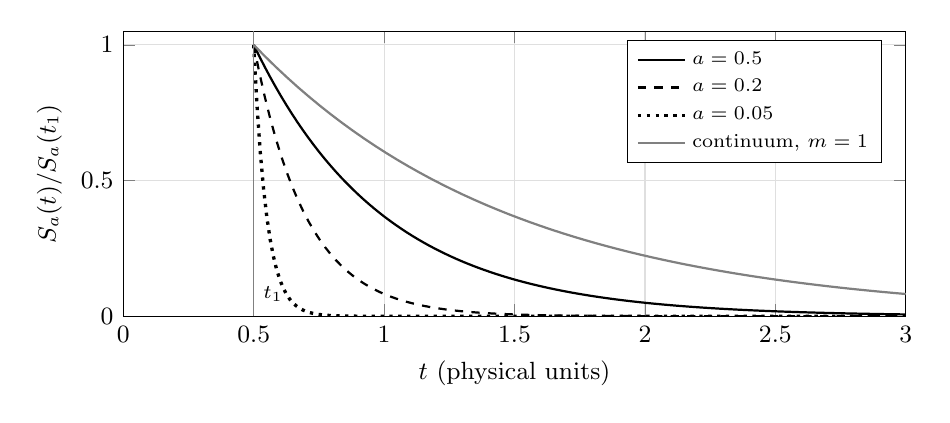
\begin{tikzpicture}
\begin{axis}[width=0.95\columnwidth,height=5.2cm,
  xmin=0,xmax=3,ymin=0,ymax=1.05,
  xlabel={$t$ (physical units)},ylabel={$S_a(t)/S_a(t_1)$},
  legend pos=north east,legend cell align=left,
  tick label style={font=\small},label style={font=\small},
  legend style={font=\scriptsize},grid=major,grid style={gray!25}]
\addplot[black,thick,domain=0.5:3,samples=120]{exp(-(x-0.5)/0.5)};
\addlegendentry{$a=0.5$}
\addplot[black,dashed,thick,domain=0.5:3,samples=120]{exp(-(x-0.5)/0.2)};
\addlegendentry{$a=0.2$}
\addplot[black,dotted,very thick,domain=0.5:3,samples=200]{exp(-(x-0.5)/0.05)};
\addlegendentry{$a=0.05$}
\addplot[gray,thick,domain=0.5:3,samples=60]{exp(-(x-0.5))};
\addlegendentry{continuum, $m=1$}
\draw[gray] (axis cs:0.5,0) -- (axis cs:0.5,1.05);
\node[font=\scriptsize,anchor=south west] at (axis cs:0.5,0.02) {$t_1$};
\end{axis}
\end{tikzpicture}
\caption{The bound $e^{-\delta(t-t_1)/a}$ of Lemma~\ref{lem:ratio} with
$\delta=1$, for three spacings, against a continuum two-point function of
mass $1$. As $a\to0$ the bound collapses onto the vertical line $t=t_1$,
whatever the renormalisation; a gapped continuum limit needs
$\delta=\delta(a)=ma$.}
\label{fig:ratio}
\end{figure}

\section{The volume obstruction}
\label{sec:volume}

\begin{lemma}
\label{lem:trace}
For $U\in\U(N)$, $|\mathrm{Re}\Tr U|\le|\Tr U|\le N$. Hence
$0\le N-\mathrm{Re}\Tr U\le2N$, $0\le S(U)\le2N|P|$ in~\eqref{eq:wilson},
and $\beta S(U)-\beta S(U')\le2N\beta|P|$ for $\beta\ge0$.
\end{lemma}

\begin{proof}
Each diagonal entry of a unitary matrix has modulus at most one; sum the
diagonal. The product of the links around a plaquette is unitary.
\end{proof}

The bound $2N$ on the oscillation of a single plaquette term is attained
for even $N$ (at $U=-I\in\SU(N)$); for odd $N$ the minimum of
$\mathrm{Re}\Tr$ on $\SU(N)$ is $-N\cos(\pi/N)$, so the oscillation is
$N(1+\cos(\pi/N))<2N$. Proposition~\ref{prop:HS} is the Holley--Stroock
lemma, proved here on a finite state space in both its Poincar\'e and its
entropy form; the argument for a compact group is the same with sums
replaced by integrals~\cite{HS87}.

\begin{proposition}[Holley--Stroock]
\label{prop:HS}
Let $\nu$ be a probability vector on a finite set, $m\le V\le M$, and
$\mu=\nu e^{-V}/Z$. Let $\Gamma\ge0$ be an energy density. If
$\Var_\nu(f)\le C\sum\nu\Gamma$ then $\Var_\mu(f)\le Ce^{M-m}\sum\mu\Gamma$.
If $g\ge0$ and $\Ent_\nu(g)\le C\sum\nu\Gamma$ then
$\Ent_\mu(g)\le Ce^{M-m}\sum\mu\Gamma$.
\end{proposition}

\begin{proof}
For a probability vector $w$, $\Var_w(f)=\min_c\sum w(f-c)^2$ and, for
$g\ge0$, $\Ent_w(g)\le\sum w\,\phi(g,c)$ for every $c>0$, with equality at
$c=\sum wg$ when that mean is positive, where
$\phi(x,c)=x\log x-x\log c-x+c\ge0$. Bound the $\mu$-average of the
nonnegative integrand by $e^{-m}/Z$ times its $\nu$-average, apply the
hypothesis, and bound $\sum\nu\Gamma\le e^{M}Z\sum\mu\Gamma$. If the
$\nu$-mean of $g$ vanishes then $g=0$ on the support of $\nu$, hence of
$\mu$, and both entropies vanish.
\end{proof}

\begin{proposition}[Volume obstruction]
\label{prop:volume}
Perturbing the product Haar measure on $\SU(N)^E$, which satisfies a
log-Sobolev inequality with a constant $\alpha_N$ independent of $E$, by the
full Wilson weight gives the constant $\alpha_Ne^{-2N\beta|P|}$, which tends
to $0$ as $|P|\to\infty$ for every $\beta>0$.
\end{proposition}

\begin{proof}
Proposition~\ref{prop:HS} with $V=\beta S$ and Lemma~\ref{lem:trace}; the
limit is $\exp(-2N\beta m)\to0$ as $m\to\infty$.
\end{proof}

Volume-uniform constants require the local transfer of~\cite{SZ92} or the
Bakry--\'Emery criterion applied to the interacting measure itself
(Section~\ref{sec:curvature}); both hold at strong coupling only.

\section{Free-energy cumulants and the Bianchi identity}
\label{sec:cumulant}

For $f_\Lambda(\beta)=-|\Lambda|^{-1}\log\int e^{-\beta S}\prod dU_e$,
\begin{equation}
f_\Lambda'(\beta)=|\Lambda|^{-1}\langle S\rangle_\beta,\qquad
f_\Lambda''(\beta)=-|\Lambda|^{-1}\Var_\beta(S),
\label{eq:derivs}
\end{equation}
and in general $f^{(n)}_\Lambda(\beta)=(-1)^{n+1}|\Lambda|^{-1}\kappa_n(S)$
with $\kappa_n$ the cumulants of $S$ under $\mu_{\Lambda,\beta}$. A bound
$|f^{(n)}_\Lambda|\le n!\,C^n$ uniform in $\Lambda$ is therefore the
statement $\kappa_n(S)=O(|\Lambda|)$, which is a decorrelation property of
the measure, and is exactly what cluster expansions prove at strong
coupling.

\begin{proposition}
\label{prop:counter}
Let $Y\in\{0,1\}$ be a fair coin and $S_n=\sum_{i=1}^n2NY$. Each term lies
in $[0,2N]$ and $\Var(S_n)/n=N^2n$, which is unbounded in $n$.
\end{proposition}

\begin{proof}
$\langle S_n\rangle=Nn$ and $\Var(S_n)=\tfrac12(Nn)^2+\tfrac12(Nn)^2$.
\end{proof}

Boundedness and nonnegativity of the local terms, the only properties used
in the analyticity arguments of the earlier manuscripts, therefore do not
bound the cumulants. Those arguments also asserted that the plaquette
variables are independent under Haar measure. They are not, in any
dimension $d\ge3$:

\begin{proposition}[Bianchi identity on a cube]
\label{prop:bianchi}
Let $\theta_e$ take values in an abelian group, and for a plaquette with
boundary edges $e_1,e_2,e_3,e_4$ let
$\theta_p=\theta_{e_1}+\theta_{e_2}-\theta_{e_3}-\theta_{e_4}$. On a unit
cube the six oriented plaquette angles sum to zero identically.
\end{proposition}

For $\U(1)$, or for the maximal torus of $\SU(N)$, the six plaquette angles
of a cube are thus linearly dependent, so they cannot be independent
uniform variables under Haar measure on links; for $\SU(N)$ the
non-abelian Bianchi identity makes a conjugated product of the six plaquette
holonomies equal to the identity. The analyticity of the
four-dimensional Wilson free energy on $(0,\infty)$ is an open problem.

\section{Running coupling and the intermediate window}
\label{sec:running}

The one-loop solution of $\mu\,dg/d\mu=-b_0g^3$ with
$b_0=11N/(48\pi^2)$ is $g^2(\mu)=1/(2b_0\log(\mu/\Lambda))$ for $\mu>\Lambda$.
It tends to $0$ as $\mu\to\infty$ and takes the value $g_*^2$ at
$\mu_*=\Lambda e^{1/(2b_0g_*^2)}$, which lies in $(\Lambda,1/a)$ whenever
$a<1/\mu_*$. Along any continuum trajectory the bare coupling $g^2(1/a)$
tends to zero, but the effective coupling at the fixed physical scale
$\mu_*$ equals $g_*^2$ at every small spacing. A renormalisation-group
analysis that integrates out scales from $1/a$ down to the mass scale must
therefore pass through every intermediate coupling. The claim of
226913, 227445 and 228638 that ``the continuum limit lies entirely inside
the Balaban regime and the intermediate coupling window is never entered''
confuses the bare coupling with the effective coupling at physical scales.
Figure~\ref{fig:running} draws the curve.

\begin{figure}[t]
\centering
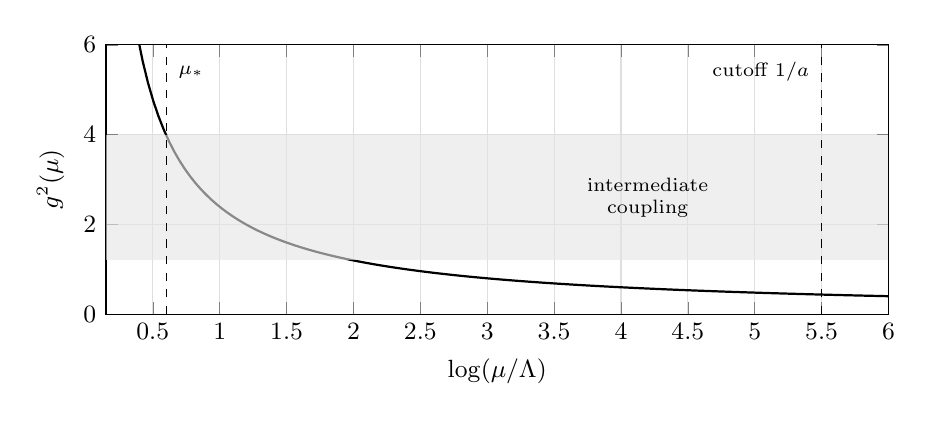
\begin{tikzpicture}
\begin{axis}[width=0.95\columnwidth,height=5.0cm,
  xmin=0.15,xmax=6,ymin=0,ymax=6,
  xlabel={$\log(\mu/\Lambda)$},ylabel={$g^2(\mu)$},
  tick label style={font=\small},label style={font=\small},
  grid=major,grid style={gray!25}]
\addplot[black,thick,domain=0.15:6,samples=150]{1/(2*0.209*x)};
\fill[gray!20,opacity=0.6] (axis cs:0.15,1.2) rectangle (axis cs:6,4);
\node[font=\scriptsize,align=center] at (axis cs:4.2,2.6) {intermediate\\coupling};
\draw[dashed] (axis cs:0.6,0) -- (axis cs:0.6,6);
\node[font=\scriptsize,anchor=west] at (axis cs:0.62,5.4) {$\mu_*$};
\draw[dashed] (axis cs:5.5,0) -- (axis cs:5.5,6);
\node[font=\scriptsize,anchor=east] at (axis cs:5.48,5.4) {cutoff $1/a$};
\end{axis}
\end{tikzpicture}
\caption{One-loop running coupling for $N=2$ ($2b_0\approx0.418$). The bare
coupling at the cutoff is small, but between the cutoff and $\Lambda$ the
curve crosses the shaded band at a scale $\mu_*$ that does not move as
$a\to0$.}
\label{fig:running}
\end{figure}

\section{Curvature of the gauge-orbit space}
\label{sec:curvature}

\begin{lemma}[Milnor]
\label{lem:milnor}
With the bi-invariant metric $\langle X,Y\rangle=-2\Tr(XY)$ on $\SU(N)$,
$\Ric=\tfrac N4\,g$.
\end{lemma}

This is correct as stated in 227159 (lines 369--393): for a bi-invariant
metric $\Ric(X,X)=-\tfrac14B(X,X)$, and the Killing form of $\mathfrak{su}(N)$
is $B(X,X)=2N\Tr X^2$. The Ricci tensor of $\SU(N)^E$ is $\tfrac N4g$ for
every $E$, so by the Bakry--\'Emery criterion the product Haar measure
satisfies the log-Sobolev inequality
\begin{equation}
\Ent(f^2)\le\frac{8}{N}\int|\nabla f|^2\,d\mathrm{Haar}
\label{eq:lsihaar}
\end{equation}
for every smooth $f$ on $\SU(N)^E$, uniformly in $E$. Gauge-invariant
functions are functions on $\SU(N)^E$, so~\eqref{eq:lsihaar} already
contains every statement about them that the orbit space could give; the
passage to $\cB=\cA/\cG$ adds nothing.

The passage as written is also incorrect. The earlier manuscripts claim
that every gauge orbit is a minimal submanifold of $\SU(N)^E$ (227159,
Lemma~\ref{lem:milnor}'s successor at lines 413--441; 227445 line 499;
228638 line 774; 226913 line 1398).

\begin{proposition}
\label{prop:notminimal}
On the one-site periodic lattice every link is a loop and the gauge group
acts by simultaneous conjugation. For $\SU(2)$ with the round metric on
$S^3$, the orbit of a configuration $(U_1,I,\dots,I)$ with
$\Tr U_1=2\cos\theta$, $0<\theta<\pi$, is a geodesic sphere of radius
$\theta$ about the identity in the first factor, with mean curvature
$2\cot\theta$. It is minimal only for $\theta=\pi/2$.
\end{proposition}

\begin{proof}
Identify $\SU(2)$ with the unit quaternions. The conjugacy class of
$\cos\theta+u\sin\theta$, $u$ a unit imaginary quaternion, is
$\{\cos\theta+v\sin\theta:|v|=1,\ v\ \text{imaginary}\}$, the set of points
at geodesic distance $\theta$ from $1$, a round two-sphere of radius
$\sin\theta$ whose principal curvatures in $S^3$ are $\cot\theta$. The
other factors are fixed points of conjugation.
\end{proof}

The proof in 227159 fails at two points. On a loop link $s(e)=t(e)=x$ the
fundamental field is $T_aU_e-U_eT_a$, which is neither left- nor
right-invariant, so $\nabla_XX\ne0$; and the mean curvature is the trace of
the second fundamental form over an orthonormal frame of the orbit, not the
sum of $\nabla_{X_{a,x}}X_{a,x}$ over the fundamental fields, whose lengths
vary along the configuration space. For an isometric action the mean
curvature of a principal orbit is the gradient of $-\log$ of the orbit
volume, which is not constant. What is true is the weighted statement: the
quotient of a space with Ricci curvature at least $K$ by a compact group
of isometries, with the push-forward of the volume measure, satisfies the
curvature-dimension condition $\mathrm{CD}(K,\infty)$~\cite{Lot03,GKMS18}.
With $K=N/4$ this is the correct form of the curvature theorem of the
earlier manuscripts; it is a statement about Haar measure and is equivalent
in content to~\eqref{eq:lsihaar} for gauge-invariant functions.

For the Wilson measure itself, the Bakry--\'Emery criterion needs
$\Ric+\beta\,\mathrm{Hess}\,S\ge K>0$. The Hessian of $S$ is bounded in
operator norm by a constant times $d-1$ per link, so this holds for
$\beta$ below a threshold of order $1/(N(d-1))$. Shen, Zhu and Zhu proved
it in this form, with 't Hooft scaling and the threshold
$|\beta|<1/(16(d-1))$ for $\SU(N)$, and derived from it the log-Sobolev
inequality, uniqueness of the infinite-volume measure and a mass
gap~\cite{SZZ23}. That is a strong-coupling theorem: it holds at fixed
$\beta$, that is at fixed lattice coupling, and by
Corollary~\ref{cor:strategy} it cannot hold with constants uniform along
the continuum trajectory.

\section{Audit of the eight manuscripts}
\label{sec:audit}

The manuscripts are 226502 (two identical copies), 226913, 227159, 227445
(two identical copies), 228638 and 229061. Line numbers refer to the source
files. Table~\ref{tab:audit} summarises; the errors are as follows.

\textbf{(E1) Uniform lattice gap.} 226502 (abstract, lines 112--121, and
Theorem lattice-gap), 226913 (lines 2256, 2309), 227445 (line 139) and
228638 (lines 216, 1679) assert $\Dlat(a)\ge\alpha_*/2$ uniformly in $a$.
By Theorem~\ref{thm:nogo} this excludes a continuum limit with a finite
gap. The same manuscripts then take $\Delta_0=\lim a\Dlat(a)$ (226502 line
121) or $\Delta_0\ge\limsup\Dlat(a)$ (227445 line 1016), mixing lattice and
physical units.

\textbf{(E2) Internal contradiction in the physical gap.} In 226502,
lines 1793--1845, the proof first obtains
$a\Dlat(a)\ge\tfrac N8(1-\varepsilon)C_{\mathrm{RS}}\Lambda^{-1}e^{-4\pi^2\beta/N}$,
which tends to $0$, and then inserts the bound
$\alpha_*\ge N\kappa_{\min}^2/(4g_{\mathrm{phys}}^2a^2)$, which tends to
$\infty$ as $a\to0$, against the definition
$\alpha_*=(N/4)(1-\varepsilon(\beta))\le N/4$ used in the same proof. The
Hessian of $-\mathrm{Re}\Tr U_p$ in the link variables does not scale like
$a^{-2}$.

\textbf{(E3) Spectral transfer.} 227445 lines 1000--1016 and 228638
line 1864 apply the Trotter--Kato theorem to operators $H_a$ that act on
different Hilbert spaces $\cH_a$ without identifying them, and the
lattice-unit gap transported by strong resolvent convergence~\cite{RS80}
becomes, in physical units, $\Dlat(a)/a\to\infty$: the spectrum of the
limit is contained in $\{0\}$, which is the ultralocal conclusion of
Theorem~\ref{thm:nogo}.

\textbf{(E4) Orbit minimality.} 227159 lines 413--441, 227445 line 499,
228638 line 774 and 226913 line 1398 assert that every gauge orbit is
minimal; Proposition~\ref{prop:notminimal} is a counterexample. The
conclusion survives only in the weighted form of
Section~\ref{sec:curvature}, for Haar measure.

\textbf{(E5) Sharpness.} 227159 line 523 states equality in
$\Gamma_2\ge\tfrac N4\Gamma$ for affine-linear $f$ on $S^3$. For the
restriction $f$ of a linear function to the round $S^3$,
$\mathrm{Hess}f=-fg$ and $\Gamma_2(f)=3f^2+2|\nabla f|^2$ in the unit
normalisation, which is not $2|\nabla f|^2$; the bound is sharp as a
spectral-gap estimate (Lichnerowicz), not pointwise.

\textbf{(E6) Analyticity of the free energy.} 227159 lines 771--799
(Lemma taylor), 226502 lines 105, 193, 2204--2249, 227445 line 799 and
228638 line 1459 bound $f^{(n)}_\Lambda$ uniformly in $\Lambda$ by treating
$|\Lambda|^{-1}S$ as a sum of independent terms under Haar measure. Three
steps fail: the derivative at $\beta_0$ is a cumulant under
$\mu_{\Lambda,\beta_0}$, not under Haar measure~\eqref{eq:derivs}; the
cumulant of the normalised sum $|\Lambda|^{-1}S$ is
$|\Lambda|^{-n}\kappa_n(S)$, so a bound on it does not bound
$|\Lambda|^{-1}\kappa_n(S)$; and the plaquette variables are not
independent (Proposition~\ref{prop:bianchi}). Without independence the
claim is false in general (Proposition~\ref{prop:counter}). A Cauchy
estimate on $\log M$ also needs $M\ne0$ on a complex disc, which is not
shown. The same argument, applied verbatim to the two-dimensional Ising
model, whose bond terms $1-\sigma_x\sigma_y$ are bounded and nonnegative,
would prove analyticity of its free energy at the critical point, against
Onsager's solution. The conclusion ``no bulk phase transition at any
$\beta>0$ and every $N\ge2$'' is unproved; for the Wilson action at large
$N$ numerical studies report bulk transitions.

\textbf{(E7) From analyticity to the Koteck\'y--Preiss criterion.} 226502
lines 106 and 228--234 infer convergence of polymer expansions at every
scale from analyticity of $f$ by ``Cauchy-estimate inversion''. The
Koteck\'y--Preiss criterion is a bound on polymer activities, which implies
analyticity and clustering; there is no converse, and analyticity of the
free energy does not imply exponential clustering.

\textbf{(E8) Avoiding intermediate coupling.} 226913 line 114, 227445
line 134 and 1124, 228638 line 1975: refuted by
Theorem~\ref{thm:D}, Section~\ref{sec:running}.

\textbf{(E9) Uniform log-Sobolev constant.}
$\alpha_*=(N/4)(1-\varepsilon(\beta))$ uniform in volume and spacing (226502
abstract; 227445 lines 127--130) is obtained by Holley--Stroock, whose
constant is $e^{-2N\beta|P|}$ (Proposition~\ref{prop:volume}); 227159
records this volume dependence correctly in its own Corollary lsi
(line~640). The step from finite volume to a uniform constant is the
Dobrushin--Stroock--Zegarlinski assembly, whose hypotheses hold at strong
coupling only, and by Corollary~\ref{cor:strategy} cannot hold uniformly
along the continuum trajectory.

\textbf{(E10) Remarks on 229061.} Its no-go theorem is correct, and is
Theorem~\ref{thm:nogo} in a weaker form. Two statements need correction:
the oscillation $2N\beta|P|$ is an upper bound, attained only for even $N$
(Section~\ref{sec:volume}); and the asserted equivalence of
$\Dlat(a)=ma+o(a)$ with a log-Sobolev constant vanishing like $a^2$ is not
a theorem, since the log-Sobolev constant is bounded by the spectral gap
but no reverse bound uniform in the volume is known.

\begin{table}[t]
\caption{Verdicts on the main claims of the eight manuscripts.}
\label{tab:audit}
\begin{ruledtabular}
\begin{tabular}{lll}
Claim & Where & Verdict\\
\hline
$\Ric_{\SU(N)}=\tfrac N4g$ & 227159:369 & true (Milnor)\\
orbits minimal & 227159:413 & false (Prop.~\ref{prop:notminimal})\\
$\mathrm{CD}(\tfrac N4,\infty)$ on $\cB$ & 227159:500 & true weighted~\cite{GKMS18}\\
LSI $\tfrac N4e^{-2N\beta|P|}$ & 227159:640 & true, not uniform\\
uniform LSI $\alpha_*$ & 226502 abs. & unproved; (E9)\\
$f$ analytic on $(0,\infty)$ & 227159:886 & unproved; (E6)\\
analyticity $\Rightarrow$ KP & 226502:233 & false implication\\
window never entered & 226913:114 & false (Thm.~\ref{thm:D})\\
$\Dlat\ge\alpha_*/2$ uniform & 226502:115 & excluded (Thm.~\ref{thm:A})\\
$\Delta_0>0$ in continuum & all but 229061 & not proved\\
no-go & 229061 & true (Thm.~\ref{thm:A})\\
\end{tabular}
\end{ruledtabular}
\end{table}

\section{What is known unconditionally}
\label{sec:known}

Reflection positivity of the Wilson measure for every compact gauge group
and every coupling, with its transfer-matrix formalism, is due to
Osterwalder and Seiler~\cite{OSei78,Sei82}. A positive transfer-matrix gap
and exponential clustering at strong coupling follow from convergent
character and cluster expansions~\cite{OSei78,Sei82,KP86}; Shen, Zhu and
Zhu obtained the log-Sobolev inequality, uniqueness and a mass gap at
strong coupling from the Bakry--\'Emery criterion and Langevin
dynamics~\cite{SZZ23}, and Nissim extended these results to $\U(N)$ in the
't Hooft regime~\cite{Nis25}. Chatterjee proved that exponential decay of
correlations under arbitrary boundary conditions, for a gauge group with
nontrivial centre, implies confinement~\cite{Cha21}; Adhikari and Cao proved
correlation decay for finite gauge groups at weak coupling~\cite{AC25}; Cao,
Nissim and Sheffield enlarged the regime in which the area law is
proved~\cite{CNS25}.

In the continuum, Ba{\l}aban's multiscale analysis proved ultraviolet
stability of four-dimensional lattice gauge theories: bounds on effective
actions and partition functions uniform in the spacing, for small bare
coupling, in a fixed physical volume~\cite{Bal87,Bal88}. Magnen,
Rivasseau and S\'en\'eor constructed four-dimensional Yang--Mills theory in
finite volume with an infrared cutoff~\cite{MRS93}. In two dimensions the
continuum Yang--Mills measure is constructed~\cite{Lev03}, and its Langevin
dynamics has been built~\cite{CCHS22}; in three dimensions Chandra,
Chevyrev, Hairer and Shen constructed the stochastic quantisation of
Yang--Mills--Higgs locally in time~\cite{CCHS24}. None of these constructs a
four-dimensional measure on $\R^4$ satisfying the Osterwalder--Schrader
axioms, and none proves a gap for one.

\section{Other claimed proofs}
\label{sec:claims}

We searched arXiv, Zenodo and PhilArchive for texts claiming the
four-dimensional mass gap. Table~\ref{tab:claims} lists those we examined,
with the mechanism stated in each abstract. We did not read every such
text in full, and the list is not exhaustive. Theorem~\ref{thm:A} applies to
any argument whose last step passes from a lattice gap uniform in lattice
units to a continuum gap; it neither repairs nor bears on arguments that
work directly in the continuum, whose gaps lie elsewhere.

\begin{table}[t]
\caption{Claimed proofs examined, with their status.}
\label{tab:claims}
\begin{ruledtabular}
\begin{tabular}{>{\raggedright\arraybackslash}p{0.32\columnwidth}>{\raggedright\arraybackslash}p{0.6\columnwidth}}
Text & Status\\
\hline
Dynin, arXiv:0903.4727 and sequels & continuum quantisation with quartic
term; Poincar\'e covariance and locality not established~\cite{Dyn09}\\
Farinelli, arXiv:1406.4177 & Coulomb-gauge construction, seventeen
versions, math.GM; not accepted~\cite{Far14}\\
Jacobsen, arXiv:2506.00284 & withdrawn by arXiv administrators~\cite{Jac25}\\
Franchi Vicer\'e, Zenodo 17966583 & finite-lattice gap by
Perron--Frobenius; reduces the problem to ``persistence of the gap'', which
in lattice units is excluded by Theorem~\ref{thm:A}~\cite{FV25}\\
Nair, arXiv:2608.10133 & outline, three dimensions; not
four-dimensional~\cite{Nai26}\\
\end{tabular}
\end{ruledtabular}
\end{table}

\section{The residual statement}
\label{sec:residual}

\begin{hypothesis}[Residual statement]
\label{hyp:R}
There exist $m\in(0,\infty)$, a trajectory $\beta=\beta(a)\to\infty$ and
renormalisations of the gauge-invariant fields such that:
\textup{(R1)} the renormalised Schwinger functions of the Wilson theory on
$a\Z^4$ converge as $a\to0$ to limits satisfying OS1--OS5;
\textup{(R2)} $\liminf_{a\to0}\Dlat(a)/a\ge m$;
\textup{(R3)} the limiting two-point functions of some gauge-invariant
field are nonzero.
\end{hypothesis}

By Lemma~\ref{lem:critical}, (R1) and (R2) make every limiting
two-point function the Laplace transform of a measure supported in
$[m,\infty)$, so by Osterwalder--Schrader reconstruction
Hypothesis~\ref{hyp:R} gives the Clay statement for the reconstructed
theory, with gap at least $m$ and, by (R3), a nontrivial theory. Theorem~\ref{thm:nogo}
shows that (R2) cannot be strengthened to a bound uniform in lattice units,
and a bound by $o(a)$ gives no gap; (R2) is the one-sided bound at the
critical scaling, and it is the Clay problem restated on the lattice.
Relative to Ba{\l}aban's programme the missing parts are the following.
Ba{\l}aban's bounds concern partition functions and effective actions in a
fixed physical volume at small bare coupling; (R1) needs the convergence of
correlation functions and the removal of the volume cutoff, which requires
control of the renormalisation-group flow at the scales where the
effective coupling is of order one (Section~\ref{sec:running}). (R2) is a
statement about exactly those scales: the lattice correlation length
$1/\Dlat(a)$ must diverge, by Corollary~\ref{cor:nogap}, but no faster
than $1/(ma)$. No method now available controls
the flow there in four dimensions.

The comparison with the Poincar\'e conjecture is instructive. Hamilton's
Ricci flow reduced that problem to the analysis of singularities, and
Perelman's noncollapsing and canonical-neighbourhood theorems classified
them, so that surgery could continue the flow. Here the
renormalisation-group flow is the analogue of the Ricci flow, Ba{\l}aban's
theorems control it where the coupling is small, and the region of order-one
coupling is the analogue of the singular set. A theorem that classified the
effective actions in that region, as Perelman's classified the singular
models, would be the step that is missing. Theorem~\ref{thm:A} shows that it
cannot be replaced by any inequality that is uniform in the spacing:
whatever controls that region must produce the divergence of the
correlation length, not exclude it.

\section{Formal verification}
\label{sec:lean}

The finite statements of this paper are checked in Lean~4 on Mathlib, in
the archive~\cite{Repo}. They are Lemma~\ref{lem:ratio},
Theorem~\ref{thm:nogo}, Lemma~\ref{lem:KL}, Corollary~\ref{cor:nogap} and
Lemma~\ref{lem:critical};
Lemma~\ref{lem:trace}, the bounds $0\le S\le2N|P|$ and the oscillation
bound $2N\beta|P|$; Proposition~\ref{prop:volume}; the Bianchi identity of
Proposition~\ref{prop:bianchi}; the variational forms of variance and
entropy and both forms of Proposition~\ref{prop:HS}; Theorem~\ref{thm:D}
with asymptotic freedom of the one-loop coupling; and
Proposition~\ref{prop:counter}. No proof is left incomplete, and each uses
only the three standard axioms of the Lean kernel (propositional
extensionality, choice and quotient soundness).

The formal statements are the abstract forms given above. The spectral
representation~\eqref{eq:spectral} is a hypothesis of the formal no-go
theorem, not a formal theorem: it is the spectral theorem for the transfer
matrix, which we quote from~\cite{OSei78,GJ87}. Likewise Milnor's formula,
the Bakry--\'Emery criterion, Proposition~\ref{prop:notminimal}, the
quotient theorem of~\cite{GKMS18} and the implications of
Corollary~\ref{cor:strategy} are proved or quoted in the text and are not
formalised; Riemannian geometry of Lie groups is not yet available in
Mathlib. Holley--Stroock is formalised on a finite state space.

\section{Conclusion}

The strategy of the eight earlier manuscripts cannot reach the Yang--Mills
mass gap, for a reason independent of the quality of its estimates: its
final inequality, a gap uniform in the lattice spacing, contradicts the
existence of a continuum limit with finite mass. Its intermediate steps
contain the errors (E1)--(E10). What it does prove correctly, a curvature
bound for Haar measure and a volume-dependent log-Sobolev constant for the
Wilson measure, is classical, and its correct strong-coupling form is the
theorem of Shen, Zhu and Zhu. The residual statement,
Hypothesis~\ref{hyp:R}, a lattice gap of at least $ma$ together with
convergence, is the Clay problem on the lattice; it requires
control of the renormalisation-group flow at order-one coupling, and it
remains open.

\section*{Data availability}

The Lean~4 source, the build configuration and the sources of this paper
are archived on Zenodo as release v1.0.0,
\href{https://doi.org/10.5281/zenodo.23444338}{doi:10.5281/zenodo.23444338}~\cite{Repo}. The Lean formalisation was prepared with
the assistance of AI tools and checked by the Lean kernel.

\section*{Conflict of interest}

The authors declare that they have no conflicts of interest and received
no funding for this work.

\raggedright
\begin{thebibliography}{99}

\bibitem{AC25}
A.~Adhikari and S.~Cao,
Correlation decay for finite lattice gauge theories at weak coupling,
Ann. Probab. \textbf{53}, 140 (2025).

\bibitem{BE85}
D.~Bakry and M.~\'Emery, Diffusions hypercontractives, in
\emph{S\'eminaire de Probabilit\'es XIX}, Lecture Notes in Mathematics
Vol.~1123 (Springer, Berlin, 1985), p.~177,
\href{https://doi.org/10.1007/BFb0075847}{doi:10.1007/BFb0075847}.

\bibitem{Bal87}
T.~Ba{\l}aban, Renormalization group approach to lattice gauge field
theories. I, Commun. Math. Phys. \textbf{109}, 249 (1987),
\href{https://doi.org/10.1007/BF01215223}{doi:10.1007/BF01215223}.

\bibitem{Bal88}
T.~Ba{\l}aban, Convergent renormalization expansions for lattice gauge
theories, Commun. Math. Phys. \textbf{119}, 243 (1988),
\href{https://doi.org/10.1007/BF01217741}{doi:10.1007/BF01217741}.

\bibitem{CNS25}
S.~Cao, R.~Nissim, and S.~Sheffield, Expanded regimes of area law for
lattice Yang--Mills theories,
\href{https://arxiv.org/abs/2505.16585}{arXiv:2505.16585}.

\bibitem{CCHS22}
A.~Chandra, I.~Chevyrev, M.~Hairer, and H.~Shen, Langevin dynamic for the
2D Yang--Mills measure, Publ. Math. IH\'ES \textbf{136}, 1 (2022).

\bibitem{CCHS24}
A.~Chandra, I.~Chevyrev, M.~Hairer, and H.~Shen, Stochastic quantisation
of Yang--Mills--Higgs in 3D, Invent. Math. \textbf{237}, 541 (2024),
\href{https://doi.org/10.1007/s00222-024-01264-2}{doi:10.1007/s00222-024-01264-2}.

\bibitem{Cha21}
S.~Chatterjee, A probabilistic mechanism for quark confinement,
\href{https://arxiv.org/abs/2006.16229}{arXiv:2006.16229}.

\bibitem{Dyn09}
A.~Dynin, Quantum Yang--Mills--Weyl dynamics in the Schr\"odinger
paradigm, \href{https://arxiv.org/abs/0903.4727}{arXiv:0903.4727}, and
later versions arXiv:1110.4682, arXiv:1205.3187, arXiv:1308.6571.

\bibitem{Far14}
S.~Farinelli, Renormalized four dimensional quantum Yang--Mills theory
and mass gap, \href{https://arxiv.org/abs/1406.4177}{arXiv:1406.4177}.

\bibitem{FV25}
C.~Franchi Vicer\'e, Yang--Mills theory on lattice and continuum:
spectral gap and existence of limit, Zenodo (2025),
\href{https://doi.org/10.5281/zenodo.17966583}{doi:10.5281/zenodo.17966583}.

\bibitem{GKMS18}
F.~Galaz-Garc\'{\i}a, M.~Kell, A.~Mondino, and G.~Sosa, On quotients of
spaces with Ricci curvature bounded below, J. Funct. Anal. \textbf{275},
1368 (2018).

\bibitem{GJ87}
J.~Glimm and A.~Jaffe, \emph{Quantum Physics: A Functional Integral Point
of View}, 2nd ed. (Springer, New York, 1987),
\href{https://doi.org/10.1007/978-1-4612-4728-9}{doi:10.1007/978-1-4612-4728-9}.

\bibitem{HS87}
R.~Holley and D.~Stroock, Logarithmic Sobolev inequalities and stochastic
Ising models, J. Stat. Phys. \textbf{46}, 1159 (1987),
\href{https://doi.org/10.1007/BF01011161}{doi:10.1007/BF01011161}.

\bibitem{Jac25}
D.~C.~Jacobsen, A constructive proof of existence and mass gap for pure
SU(3) Yang--Mills in four-dimensional space-time,
\href{https://arxiv.org/abs/2506.00284}{arXiv:2506.00284} (withdrawn).

\bibitem{JW00}
A.~Jaffe and E.~Witten, Quantum Yang--Mills theory, Clay Mathematics
Institute Millennium Prize problem description (2000).

\bibitem{KP86}
R.~Koteck\'y and D.~Preiss, Cluster expansion for abstract polymer models,
Commun. Math. Phys. \textbf{103}, 491 (1986),
\href{https://doi.org/10.1007/BF01211762}{doi:10.1007/BF01211762}.

\bibitem{Lev03}
T.~L\'evy, Yang--Mills measure on compact surfaces, Mem. Amer. Math. Soc.
\textbf{166}, no.~790 (2003).

\bibitem{Lot03}
J.~Lott, Some geometric properties of the Bakry--\'Emery--Ricci tensor,
Comment. Math. Helv. \textbf{78}, 865 (2003).

\bibitem{MRS93}
J.~Magnen, V.~Rivasseau, and R.~S\'en\'eor, Construction of $YM_4$ with an
infrared cutoff, Commun. Math. Phys. \textbf{155}, 325 (1993).

\bibitem{Mil76}
J.~Milnor, Curvatures of left invariant metrics on Lie groups, Adv. Math.
\textbf{21}, 293 (1976),
\href{https://doi.org/10.1016/S0001-8708(76)80002-3}{doi:10.1016/S0001-8708(76)80002-3}.

\bibitem{Nai26}
V.~P.~Nair, Towards a proof of mass gap in 3d Yang--Mills theory,
\href{https://arxiv.org/abs/2608.10133}{arXiv:2608.10133}.

\bibitem{Nis25}
R.~Nissim, $\U(N)$ lattice Yang--Mills in the 't Hooft regime,
\href{https://arxiv.org/abs/2510.22788}{arXiv:2510.22788}.

\bibitem{OS73}
K.~Osterwalder and R.~Schrader, Axioms for Euclidean Green's functions,
Commun. Math. Phys. \textbf{31}, 83 (1973),
\href{https://doi.org/10.1007/BF01645738}{doi:10.1007/BF01645738}.

\bibitem{OS75}
K.~Osterwalder and R.~Schrader, Axioms for Euclidean Green's functions.
II, Commun. Math. Phys. \textbf{42}, 281 (1975),
\href{https://doi.org/10.1007/BF01608978}{doi:10.1007/BF01608978}.

\bibitem{OSei78}
K.~Osterwalder and E.~Seiler, Gauge field theories on a lattice, Ann.
Phys. (N.Y.) \textbf{110}, 440 (1978),
\href{https://doi.org/10.1016/0003-4916(78)90039-8}{doi:10.1016/0003-4916(78)90039-8}.

\bibitem{RS80}
M.~Reed and B.~Simon, \emph{Methods of Modern Mathematical Physics I:
Functional Analysis}, revised ed. (Academic Press, New York, 1980).

\bibitem{Repo}
D.~Bhattacharjee and U.~Bhattacharya, Spacing-uniform lattice inequalities
cannot produce the Yang--Mills mass gap: paper, audit and Lean certificate,
Zenodo, release v1.0.0 (2026),
\href{https://doi.org/10.5281/zenodo.23444338}{doi:10.5281/zenodo.23444338}.

\bibitem{Sei82}
E.~Seiler, \emph{Gauge Theories as a Problem of Constructive Quantum Field
Theory and Statistical Mechanics}, Lecture Notes in Physics Vol.~159
(Springer, Berlin, 1982),
\href{https://doi.org/10.1007/3-540-11559-5}{doi:10.1007/3-540-11559-5}.

\bibitem{SZZ23}
H.~Shen, R.~Zhu, and X.~Zhu, A stochastic analysis approach to lattice
Yang--Mills at strong coupling, Commun. Math. Phys. \textbf{400}, 805
(2023), \href{https://doi.org/10.1007/s00220-022-04609-1}{doi:10.1007/s00220-022-04609-1}.

\bibitem{SZ92}
D.~Stroock and B.~Zegarlinski, The logarithmic Sobolev inequality for
discrete spin systems on a lattice, Commun. Math. Phys. \textbf{149}, 175
(1992), \href{https://doi.org/10.1007/BF02096629}{doi:10.1007/BF02096629}.

\bibitem{Wil74}
K.~G.~Wilson, Confinement of quarks, Phys. Rev. D \textbf{10}, 2445 (1974),
\href{https://doi.org/10.1103/PhysRevD.10.2445}{doi:10.1103/PhysRevD.10.2445}.

\end{thebibliography}

\end{document}
